\documentclass[12pt]{article} 
\usepackage[utf8]{inputenc}
\usepackage{geometry}
\geometry{letterpaper}
\usepackage{graphicx} 
\usepackage{parskip}
\usepackage{booktabs}
\usepackage{array} 
\usepackage{paralist} 
\usepackage{verbatim}
\usepackage{subfig}
\usepackage{fancyhdr}
\usepackage{sectsty}

\pagestyle{fancy}
\renewcommand{\headrulewidth}{0pt} 
\lhead{}\chead{}\rhead{}
\lfoot{}\cfoot{\thepage}\rfoot{}

%%% SECTION TITLE APPEARANCE
\allsectionsfont{\sffamily\mdseries\upshape} 

%%% ToC (table of contents) APPEARANCE
\usepackage[nottoc,notlof,notlot]{tocbibind} 
\usepackage[titles,subfigure]{tocloft}
\renewcommand{\cftsecfont}{\rmfamily\mdseries\upshape}
\renewcommand{\cftsecpagefont}{\rmfamily\mdseries\upshape} %

\usepackage{amsmath}
\usepackage{amssymb}
\usepackage{empheq}
\usepackage{xcolor}
\renewcommand{\L}[1]{\mathcal{L}\{#1\}}
\newcommand{\ans}[1]{\boxed{\text{#1}}}
\newcommand{\vecs}[1]{\langle #1\rangle}
\renewcommand{\hat}[1]{\widehat{#1}}
\newcommand{\F}[1]{\mathcal{F}(#1)}
\renewcommand{\P}{\mathbb{P}}
\newcommand{\R}{\mathbb{R}}
\newcommand{\qed}{\quad \blacksquare}
\newcommand{\brak}[1]{\langle #1 \rangle}

\title{APMA 0360: Homework 8}
\author{Milan Capoor}
\date{7 April 2023}

\begin{document}
\maketitle
\section*{Problem 1}
Assuming only that the cosine functions are orthogonal,
\begin{enumerate}
    \item Derive Parseval's identity for the following expansion on $(0, \pi)$
    \[1 = \sum_{m=0}^\infty A_m \cos\left(\left(\frac{2m+1}{2}\right)x\right)\]
    
    \color{blue}
    Letting $f(x) = 1$ and taking the square norm of each side, 
    \[||1||^2 = \int_0^\pi f(x)^2 \; dx = \left|\left|\sum_{m=0}^\infty A_m \cos\left(\left(\frac{2m+1}{2}\right)x\right)\right|\right|^2\]
    But since $\{\cos(mx)\}$ is orthogonal, 
    \begin{align*}
        \left|\left|\sum_{m=1}^\infty A_m \cos\left(\left(\frac{2m+1}{2}\right)x\right)\right|\right|^2 &= \sum_{m=1}^\infty \left|\left|A_m \cos\left(\left(\frac{2m+1}{2}\right)x\right)\right|\right|^2\\
        &= \sum_{m=1}^\infty |A_m|^2\; \left|\left|\cos\left(\left(\frac{2m+1}{2}\right)x\right)\right|\right|^2\\
        &= \sum_{m=1}^\infty |A_m|^2\; \left(\cos\left(\left(\frac{2m+1}{2}\right)x\right) \cdot \cos\left(\left(\frac{2m+1}{2}\right)x\right)\right)\\
        &= \sum_{m=1}^\infty |A_m|^2 \int_0^\pi \cos^2 \left(\left(\frac{2m+1}{2}\right)x\right) \; dx
    \end{align*}

    Evaluating the integral:
    \begin{align*}
        \int_0^\pi \cos^2 \left(\left(\frac{2m+1}{2}\right)x\right) \; dx &= \int_0^\pi 1 - \sin^2\left(\left(\frac{2m+1}{2}\right)x\right)\; dx\\
        &= \pi - \int_0^\pi \frac{1}{2} - \frac{1}{2}\cos\left(\left(2m+1\right)x\right)\; dx\\
        &= \frac{\pi}{2} - \frac{1}{2} \int_0^\pi \cos((2m + 1)x)\; dx\\
        &= \frac{\pi}{2} - \frac{1}{2}\left[\frac{\sin((2m + 1)x)}{2m + 1}\right]_0^\pi\\
        &= \frac{\pi}{2} - \frac{1}{2}(\frac{\sin(2\pi m + \pi)}{2m + 1} - 0) = \frac{\pi}{2} + \frac{\sin(2\pi m)}{4m + 2} = \frac{\pi}{2}
    \end{align*}
    Which finally gives 
    \[\int_0^\pi f(x)^2\; dx = \sum_{m=0}^\infty |A_m|^2 \cdot \frac{\pi}{2} \]
    or 
    \[\sum_{m=0}^\infty |A_m|^2 = \frac{2}{\pi} \int_0^\pi f(x)^2 \; dx\]
    which is Parseval's identity. $\qed$

    \color{black}
    \item Use (1) to calculate the sum 
    \[\sum_{m=0}^\infty \frac{1}{(2m+1)^2} = 1 + \frac{1}{3^2} + \frac{1}{5^2} + ...\]

    \color{blue}
    \[A_m = \frac{1 \cdot \cos\left(\left(\frac{2m+1}{2}\right)x\right)}{\cos\left(\left(\frac{2m+1}{2}\right)x\right) \cdot \cos\left(\left(\frac{2m+1}{2}\right)x\right)} = \frac{\int_0^\pi\cos\left(\left(\frac{2m+1}{2}\right)x\right)\; dx}{\int_0^\pi \cos^2\left(\left(\frac{2m+1}{2}\right)x\right)\; dx}\]
    From part a, 
    \[\int_0^\pi \cos^2\left(\left(\frac{2m+1}{2}\right)x\right)\; dx = \frac{\pi}{2}\]
    and 
    \[\int_0^\pi\cos\left(\left(\frac{2m+1}{2}\right)x\right)\; dx = \left[\frac{2}{2m+1}\sin\left(\frac{2m+1}{2}x\right)\right]_0^\pi = \frac{2}{2m+1}(-1)^m\]
    so 
    \[A_m = \frac{2(-1)^m / (2m+1)}{\pi/2} = \frac{4(-1)^m}{\pi(2m + 1)}\]
    Then again from (a), 
    \begin{gather*}
        |1|^2 = \frac{\pi}{2}\sum_{m=0}^\infty |A_m|^2 = \frac{\pi}{2}\sum_{m=0}^\infty \left|\frac{4(-1)^m}{\pi (2m +1)}\right|^2 = \frac{\pi}{2} \cdot \frac{16}{\pi^2} \sum_{m=0}^\infty \frac{1}{(2m+1)^2}\\
        \pi = \frac{8}{\pi} \sum_{m=0}^\infty \frac{1}{(2m+1)^2}
    \end{gather*}
    Then at long last, 
    \[\boxed{\sum_{m=0}^\infty \frac{1}{(2m +1)^2} = \frac{\pi^2}{8}}\]
\end{enumerate}

\pagebreak
\section*{Problem 2:}
\begin{enumerate}
    \item Find the Fourier sine series of $f(x) = x^3$ on $(0, \pi)$
    
    \color{blue}
    For 
    \[x^3 = \sum_{m=1}^\infty A_m \sin(mx)\]
    we have 
    \[A_m = \frac{\int_0^\pi x^3\sin(mx)\; dx}{\int_0^\pi \sin^2(mx)\; dx} = \frac{2}{\pi} \int_0^\pi x^3\sin(mx)\;dx\]

    Using Tabular integration,
    \[\begin{array}{ccc}
        x^3 & & \sin(mx)\\
        & \searrow & \\
        -3x^2 & & -\cos(mx)/m\\
        & \searrow & \\
        6x & & -\sin(mx)/m^2\\
        & \searrow & \\
        -6 & & \cos(mx)/m^3\\
        & \searrow & \\
        0 & & \sin(mx)/m^4
    \end{array}\]
    so 
    \begin{align*}
       \int_0^\pi x^3\sin(mx)\;dx &= \left[-x^3 \frac{\cos(mx)}{m} + 3x^2 \frac{\sin(mx)}{m^2} + 6x\frac{\cos(mx)}{m^3} - 6\frac{\sin(mx)}{m^4}\right]_0^\pi\\
       &= -\pi^3 \frac{(-1)^m}{m} + 6\pi\frac{(-1)^m}{m^3}\\
       &= \pi^3 \frac{(-1)^{m+1}}{m} + 6\pi \frac{(-1)^m}{m^3}
    \end{align*}
    and 
    \[A_m = 2\pi^2 \frac{(-1)^{m+1}}{m} + 12\frac{(-1)^m}{m^3}\]
    so 
    \[\boxed{x^3 = \sum_{m=1}^\infty (2\pi^2 \frac{(-1)^{m+1}}{m} + 12\frac{(-1)^m}{m^3})\sin(mx)}\]

    \color{black}
    \item Apply Parseval's identity to (1) to find
    \[\sum_{m=1}^\infty \frac{1}{m^6}\]

    \textbf{Hint:} use without proof the fact that 
    \[\sum_{m=1}^\infty \frac{1}{m^2} = \frac{\pi^2}{6} \text{ and } \sum_{m=1}^\infty \frac{1}{m^4} = \frac{\pi^4}{90}\]

    \color{blue}
    Parseval's identity states that 
    \[\sum_{m=1}^\infty |A_m|^2 = \frac{2}{\pi} \int_0^\pi f(x)^2 \; dx\]
    Here, 
    \[\begin{cases}
        A_m = 2\pi^2 \frac{(-1)^{m+1}}{m} + 12\frac{(-1)^m}{m^3}\\
        f(x) = x^3
    \end{cases}\]
    So, 
    \begin{align*}
        |A_m|^2 &= \left| 2\pi^2 \frac{(-1)^{m+1}}{m} + 12\frac{(-1)^m}{m^3}\right|^2 \\
        &= (\frac{2}{m}(-1)^m)^2(-\pi^2 + \frac{6}{m^2})^2\\
        &= \frac{4}{m^2}(\pi^4 - 12\frac{\pi^2}{m^2} + \frac{36}{m^2})\\
        &= \frac{4\pi^4}{m^2} - \frac{48\pi^2}{m^4} + \frac{144}{m^6}
    \end{align*}    and 
    \[\frac{2}{\pi}\int_0^\pi x^6 \; dx = \frac{2}{\pi} \cdot \frac{\pi^7}{7} = \frac{2\pi^6}{7}\]
    Plugging back into Parseval's, 
    \[\sum_{m=1}^\infty \frac{4\pi^4}{m^2} - \frac{48\pi^2}{m^4} + \frac{144}{m^6} = \frac{2\pi^6}{7}\]
    \[4\pi^4 \sum_{m=1}^\infty \frac{1}{m^2} - 48\pi^2\sum_{m=1}^\infty \frac{1}{m^4} + 144\sum_{m=1}^\infty \frac{1}{m^6} = \frac{2\pi^6}{7}\]
    \[4\pi^4(\frac{\pi^2}{6}) - 48\pi^2 (\frac{\pi^4}{90}) + 144\sum_{m=1}^\infty \frac{1}{m^6} = \frac{2\pi^6}{7}\]
    So,
    \begin{align*}
        \sum_{m=1}^\infty \frac{1}{m^6} &= \frac{1}{144}\left(\frac{2}{7} - \frac{4}{6} + \frac{48}{90}\right)\pi^6\\
        &= \boxed{\frac{\pi^6}{945}}
    \end{align*}
\end{enumerate}

\pagebreak 
\section*{Problem 3:}
In this problem, you do NOT have to calculate the coefficients.

Hint: For (2), since the Fourier cosine series is an even function, you first have to reflect the graph of f about the y-axis to get a function on $(-1, 1)$ and then apply the usual rules. For (3) it's the same thing but this time you reflect the graph about the origin to get an odd function since the Fourier sine series is odd.

\begin{enumerate}
    \item Let $f(x) = e^x$ in $(-1, 1)$ and draw the graph of the full Fourier series of f(x) on all of $\R$
    
    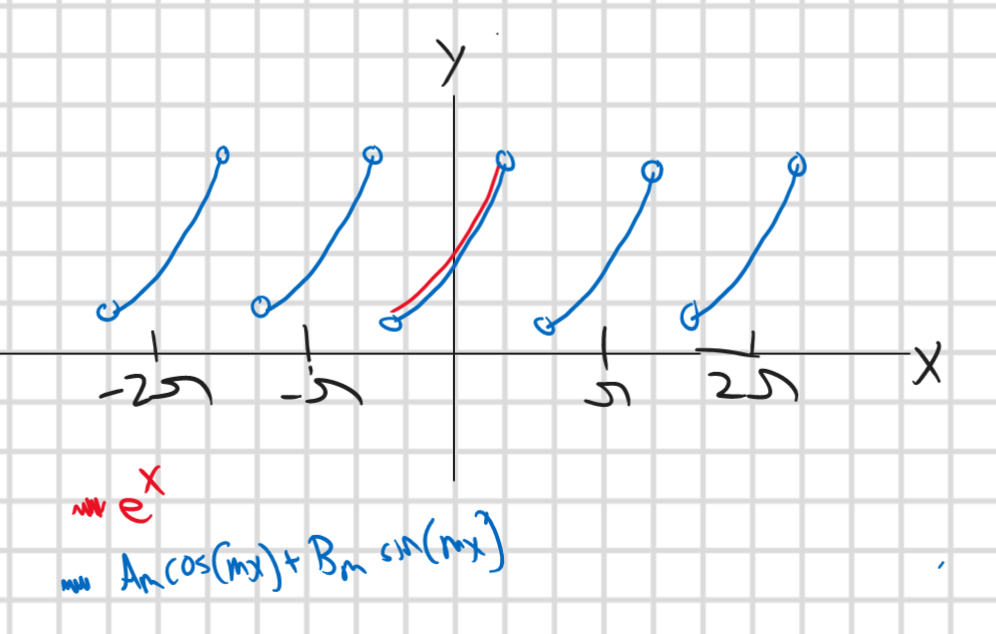
\includegraphics[width=0.8\textwidth]{Images/full fourier.png}
    
    \pagebreak
    \item Let $f(x) = e^x$ in $(0, 1)$ and draw the graph of the Fourier cosine series of f(x) on all of $\R$
    
    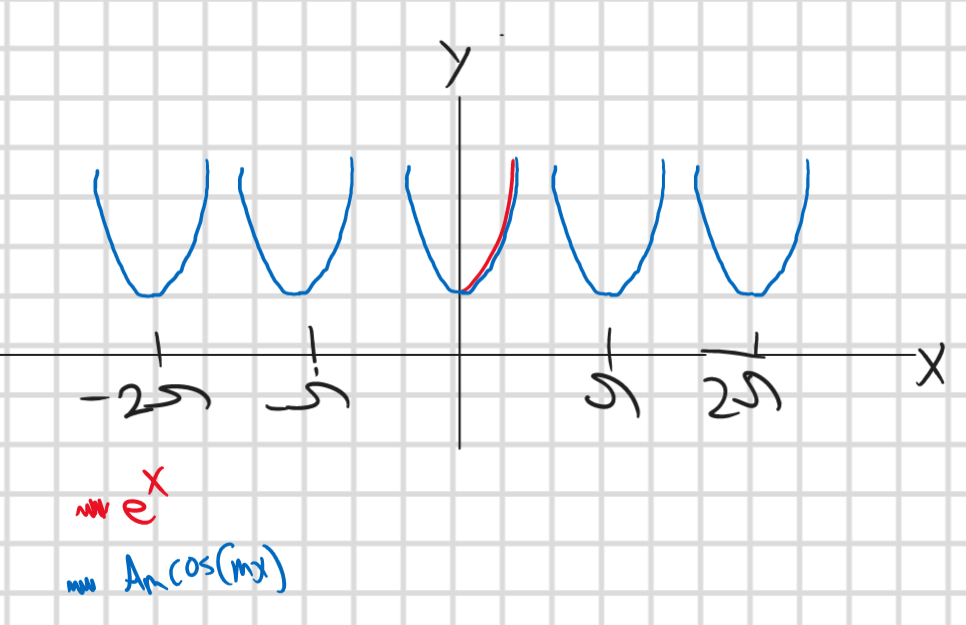
\includegraphics[width=0.8\textwidth]{Images/cos.png}

    \item Let $f(x) = e^x$ in $(0, 1)$ and draw the graph of the Fourier sine series of f(x) on all of $\R$
     
    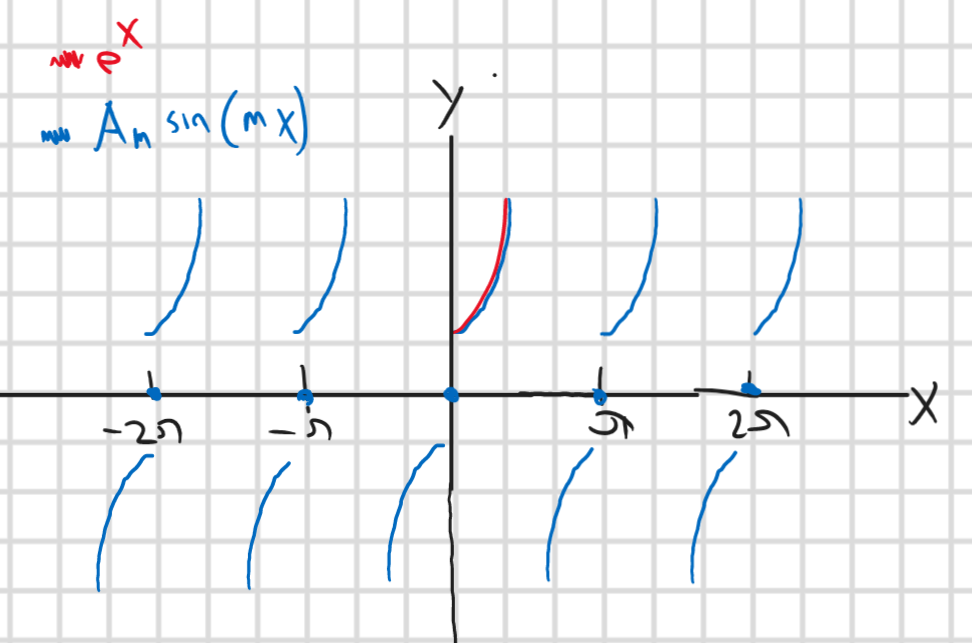
\includegraphics[width=0.8\textwidth]{Images/sin.png}
    
\end{enumerate}


\pagebreak
\section*{Problem 4:} 
\begin{empheq}[box=\fbox]{gather*}
    \\
    \; \text{\textbf{Definition:}} \qquad \qquad \qquad\qquad\qquad\qquad\\
    \text{We say $u = u(x, y)$ is \emph{subharmonic} if} \quad \\
    -(u_{xx} + u_{yy}) \leq 0\\
\end{empheq}

\begin{enumerate}
    \item Suppose u is harmonic and $f'' \geq 0$ and let $v = f(u)$ Show that v is subharmonic
    
    \color{blue}
    \begin{gather*}
        v = f(u)\\
        v_{x} = f'(u)\cdot u_x\\
        v_{xx} = f''(u)\cdot u_x^2 + f'(u) \cdot u_{xx}\\
        v_y = f'(u) \cdot u_y\\
        v_{yy} = f''(u) \cdot u_y^2 + f'(u) \cdot u_{yy}
    \end{gather*} 
    Then notice that 
    \begin{align*}
        v_{xx} + v_{yy} &=  f''(u)\cdot u_x + f'(u) \cdot u_{xx} + f''(u) \cdot u_y + f'(u) \cdot u_{yy}\\
        &= f''(u) \cdot (u_x^2 + u_y^2) + f'(u)\cdot (u_{xx} + u_{yy})
    \end{align*}
    But if u is harmonic, 
    \[u_{xx} + u_{yy} = 0\]
    so 
    \[v_{xx} + v_{yy} = f''(u) \cdot (u_x + u_y).\]

    Because $f'' \geq 0$, we know that 
    \[v_{xx} + v_{yy} \geq u_x^2 + u_y^2\]
    And as the RHS is a sum of squares it is non-negative so 
    \[v_{xx} + v_{yy} \geq 0\]
    and 
    \[-(v_{xx} + v_{yy}) \leq 0\]
    so $v$ is subharmonic. $\qed$
    \color{black}

    \item Suppose u is harmonic and let $w = (u_x)^2 + (u_y)$. Show that w is subharmonic
    
    \color{blue}
    Taking the derivatives of $w$:
    \begin{gather*}
        w_x = 2u_x \cdot u_{xx} + u_{yx}\\ 
        w_{xx} = 2u_{xx} \cdot u_{xx}  + 2u_x \cdot u_{xxx} + u_{yxx}\\
        w_y = 2u_x \cdot u_{xy} + u_{yy}\\
        w_{yy} = 2u_{xy} \cdot u_{xy} + 2u_x \cdot u_{xyy} + u_{yyy}
    \end{gather*}
    So 
    \begin{align*}
        w_{xx} + w_{yy} &= 2u_{xx} \cdot u_{xx}  + 2u_x \cdot u_{xxx} + u_{yxx} +  2u_{xy} \cdot u_{xy} + 2u_x \cdot u_{xyy} + u_{yyy}\\
        &= 2u_{xx}^2 + 2u_x(u_{xxx} + u_{xyy}) + u_{yxx} + 2u_{xy}^2 + u_{yyy}\\
        &= 2u_{xx}^2 + 2u_{xy}^2 + 2u_x(u_{xx} + u_{yy})_x + (u_{xx} + u_{yy})_y
    \end{align*}
    Then as $u$ is harmonic, $u_{xx} + u_{yy} = 0$ and 
    \[w_{xx} + w_{yy} = 2(u_{xx}^2 + u_{xy}^2)\]
    as the RHS is a sum of squares, though, it is non-negative so 
    \[w_{xx} + w_{yy} \geq 0\]
    and 
    \[-(w_{xx} + w_{yy}) \leq 0\]
    showing that $w$ is subharmonic. $\qed$ 
\end{enumerate}

\pagebreak
\subsection*{Problem 5:}
Same setting as the derivation of the heat equation, but this time, instead of a line, you have a grid where the particle can jump left/right but also up/down (but not diagonally) all with equal probability.

Show that$ u = u(x, y, t)$ solves the 2D heat equation
\[u_t = D (u_{xx }+ u_{yy})\]

\textbf{Note:} Here once again you choose $\tau$ in terms of h so that in the limit you get D. Just beware that the definition of D will be slightly different than from the 1D heat equation

\color{blue}
Let $u = u(x, y, t)$ be the concentration of particles at each point on a metal plate. We consider a small interval around $(x, y)$ where as $t \to t + \tau$, each particle moves up, down, left, or right with equal probability. Then, the number of particles at $(x, y)$ at $t = t + \tau$ is equal to the number of particles at $(x, y, t)$ plus the change:
\[h^2u(x, y, t + \tau) = h^2u(x, y, t) + I(x, y, t) + O(x, y, t)\]
where
\begin{align*}
    I(x, y, t) &= \frac{h^2}{4}\left(u(x - h, y, t) + u(x, y + h, t) + u(x + h, y, t) + u(x, y - h, t)\right)\\
    O(x, y, t) &= h^2u(x, y, t)
\end{align*} 
So 
\begin{align*}
    h^2u(x, y, t + \tau) - h^2u(x, y, t) &= \frac{h^2}{4}\left(u(x - h, y, t) + u(x + h, y, t)\right)\\
    &+ \frac{h^2}{4}\left(u(x, y - h, t) + u(x, y + h, t)\right)\\
    & - h^2u(x, y, t)
\end{align*}
\begin{align*}
    u(x, y, t + \tau) - u(x, y, t) &= \frac{h^2}{4}\cdot \frac{u(x- h, y, t) - 2u(x, y, t) + u(x + h, y, t)}{h^2}\\
    &+ \frac{h^2}{4}\cdot\frac{u(x, y - h, t) - 2u(x, y, t) + u(x, y + h, t)}{h^2}
\end{align*}
Then for small h, this is just the limit definition of the second derivative so 
\[u(x, y, t + \tau) - u(x, y, t) = \frac{h^2}{4}(u_{xx} + u_{yy})\]
Divide by $\tau$ to get
\[\frac{u(x, y, t + \tau) - u(x, y, t)}{\tau} = \frac{h^2}{4\tau}(u_{xx} + u_{yy})\]
Then for small $\tau$, this is also a derivative and 
\[u_t = \frac{h^2}{4\tau}(u_{xx} + u_{yy})\]
Let $D = \frac{h^2}{4\tau}$ and we have the 2D heat equation 
\[u_t = D(u_{xx} + u_{yy}) \qed\]

\end{document}